\documentclass[12pt]{article}
\usepackage{amsmath,amssymb}
\usepackage{graphicx}
\usepackage{booktabs}
\newtheorem{theorem}{Theorem}
\newtheorem{proposition}[theorem]{Proposition}
\newtheorem{corollary}[theorem]{Corollary}
\newtheorem{lemma}[theorem]{Lemma}
\usepackage{fullpage}
\usepackage{parskip}
 \usepackage{relsize}
\usepackage{dcolumn}
\usepackage{amsfonts}
\usepackage{multicol}
\DeclareMathSizes{11}{30}{20}{12}
\newcommand{\Z}{\mathbb{Z}}

\renewcommand{\labelenumi}{(\alph{enumi})}
\begin{document}

\centerline{\bf Math Camp - Homework 3}


\bigskip

\noindent \textbf{1.} 
\begin{enumerate}
\item Sketch the graph of a function (any function you like, no need to specify a functional form) that is continuous on [0,3] and has the following properties: an absolute maximum at 0, an absolute minimum at 3, a local minimum at 1 and a local maximum at 2.
\item Do the same for another function with the following properties: 2 is a critical number, but there is no local minimum and no  local maximum.
\end{enumerate}

\noindent \textbf{2.} Find the critical values of these functions:\\

\begin{multicols}{2}
\begin{enumerate}
\item $f(x) = 5x^{3/2} - 4x$
\item $s(t) = 3t^4 + 4t^3 - 6t^2$
\item $f(r) = \frac{r}{r^2 + 1}$
\item $h(x) = x log(x)$
\end{enumerate}
\end{multicols}

\noindent \textbf{3.} Find the absolute minimum and absolute maximum values of the functions on the given interval:\\

\begin{multicols}{2}
\begin{enumerate}
\item $f(x) = 3x^2 - 12x + 5, [0,3] $
\item $f(t) = t\sqrt{4 - t^2}, [-1,4]$
\item $s(x) = x - ln(x), [1/2, 2]$
\item $h(p) = 1 - e^{-p}, [0,1000]$
\end{enumerate}
\end{multicols}

\noindent \textbf{4.} Prove that the function $f(x) = x^5 + x^3 + x + 1$ has no local maximum and no local minimum\\

\noindent \textbf{5.} Does a continuous, differentiable function exist on [0,2] such that f(0) = -1, f(2) = 4, and f'(x) $\le 2 \  \forall$ x?\\
Use the mean value theorem to explain your answer.  

\pagebreak

\noindent \textbf{6.} A friend shows you this graph of a function g(x). 

\begin{figure}[!ht]
\centering
\caption{Graph of g(x)}
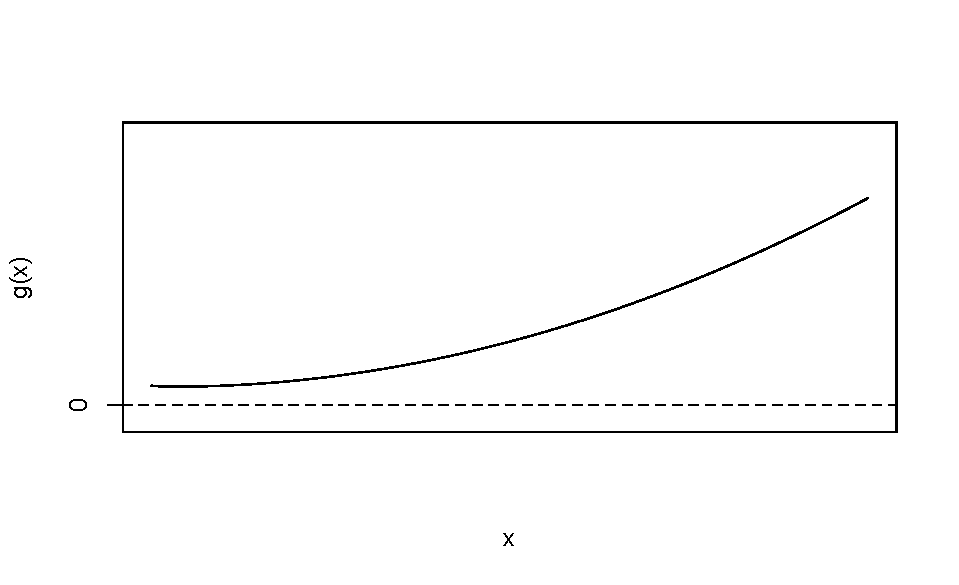
\includegraphics[height=2.5in, width=3.5in]{function1.pdf}
\end{figure}


Which of the following could be a graph of g'(x)? For each graph explain why or why not it might be the derivative of g(x). 

\begin{figure}[!ht]
\centering
\caption{Potential Derivatives}
\includegraphics[height=4in, width=6in]{examples.pdf}
\end{figure}

\pagebreak

What about if Figure 3 was the graph of g(x)? Which of the graphs might potentially be the derivative of g(x) then?

\begin{figure}[!ht]
\centering
\caption{Graph of g(x)}
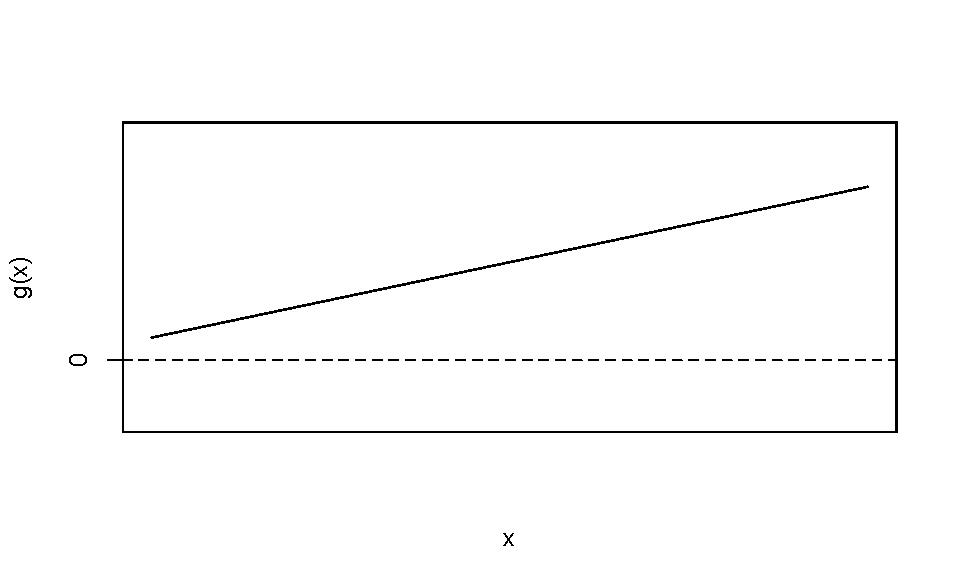
\includegraphics[height=2.5in, width=3.5in]{function2.pdf}
\end{figure}

\noindent \textbf{7.}
Suppose we were interested in learning about how years of schooling affect the probability that a person turns out to vote. To simplify things, let's say we just have one observation of each variable. Let $Y$ be our single observation of the dependent variable (whether or not a person turns out to vote) and $X$ be our single observation of the independent variable, (the number of years of education that same person has). We believe that the process used to generate our data takes the following form:

\bigskip
\begin{eqnarray*}
Y&=&\beta X + \epsilon\\
 \end{eqnarray*}
 
 where $\epsilon$ is an error term. We include this error term because we think random occurrences in the world will mean our model produces estimates that are slightly wrong sometimes, but we believe that on average, this model accurately relates $X$ to $Y$. We observe the values of $X$ and $Y$, but what about $\beta$? How do we know the value of $\beta$ that best approximates this relationship, i.e., what's the slope of this line?
 
 There are different criteria we could use, but a popular choice is the method of least squares. In this process, we solve for the value of $\beta$ that minimizes the sum of squared errors, $\epsilon^2$, in our data. Using the tools of minimization we've been practicing, find the value of $\beta$ that minimizes this quantity. (Hint: In this case there is only one observation, so the sum of squared errors is equal to the single error squared.)

\end{document}